\documentclass{article}
\usepackage[english]{babel}
\usepackage[utf8]{inputenc}

% align for equations
\usepackage{amsfonts}
\usepackage{mathtools}

% Table formatting
\usepackage{booktabs}

% References and Bibliography
\usepackage[natbibapa]{apacite}
\usepackage{natbib}
\bibliographystyle{apacite}
\usepackage[hidelinks]{hyperref}
\usepackage{cleveref}
\Crefname{section}{Section}{Sections}
\crefname{section}{Section}{Sections}
\Crefname{figure}{Figure}{Figures}
\crefname{figure}{Figure}{Figures}
\Crefname{table}{Table}{Table}
\crefname{table}{Table}{Table}
\Crefname{equation}{Equation}{Equation}
\crefname{equation}{Equation}{Equation}

\newcommand{\documentlanguage}{english}  % Change to german if needed

\let\oldquote\quote
\let\endoldquote\endquote
\renewenvironment{quote}[2][]
  {\if\relax\detokenize{#1}\relax
     \def\quoteauthor{#2}%
   \else
     \def\quoteauthor{#2~---~#1}%
   \fi
   \oldquote}
  {\par\nobreak\smallskip\hfill(\quoteauthor)%
   \endoldquote\addvspace{\bigskipamount}}

\begin{document}
\begin{otherlanguage}{\documentlanguage}
\begin{titlepage}
\begin{center}
	\vspace{3em}	
    {\Huge\bfseries Seminar - \textit{Critical Topics in AI}\par}
    \vspace{2em}
    {\huge \textit{AGI - Benchmarks, Feasibility, Implications} \par}
    \vspace{3em}
    Author\\
	\vspace{1em}
    {\Large \textit{Frederik Schittny}\par}
    \vspace{1em}
    Matrikelnummer: \textit{2612609}\\
    \vspace{3em}
    Date:\\
	\vspace{1em}
    Karlsruhe, \today
\end{center}
\end{titlepage}
\newpage
\setcounter{page}{1}
\pagenumbering{Roman}
\section*{Abstract}
The concept of human-level or artificial general intelligence (AGI) has been a much-anticipated technological goal for many years.
Throughout the history of artificial intelligence, experts have repeatedly and incorrectly predicted AGI's short-term achievement.
But despite many impactful advancements in the field of artificial intelligence, no clear path towards AGI is known decades after its inception.
In this report, we demonstrate that the main problem in the development of AGI lies in its ambiguous definition.
We relate the vagueness of the term AGI back to its basis in the concept of intelligence and point out how the resulting ambiguity allows for individual and subjective understandings of AGI.
Additionally, we highlight the impact of this ambiguity on benchmarking strategies, technical approaches for implementation, the prognosis of development timelines, and predictions of impacts related to AGI.
As a consequence of AGI's intrinsic ambiguity, no targeted development of AGI is possible without a better understanding of the underlying concept of intelligence as a whole.
Nevertheless, discussions on this topic rarely address the clarification of subjective conceptions of AGI or acknowledge the lack of a universal AGI definition.
\newpage
\tableofcontents
\newpage
\setcounter{page}{1}
\pagenumbering{arabic}
\section{Introduction}\label{sec:introduction}

Artificial general intelligence (AGI) is a topic that has gained increasing interest in both research and public discussion in recent years.
The main driver of this increasing interest was the release and widespread adoption of ChatGPT-3 and subsequent large language models (LLMs).
The rapid improvement of these LLMs with techniques like chain of thought reasoning, tool usage, and independent agentic action taking has brought up the question of how this new advancement in the broader field of artificial intelligence (AI) is related to the concept of AGI.
Several of the companies developing some of the most popular LLMs, including OpenAI, Google, Anthropic, and Meta, have stated AGI as a long-term goal of their scientific efforts.\\

Despite the recent increase in focus on AGI, the concept is not new.
Concepts of machines exhibiting intelligence equivalent to, or even surpassing, that of humans can not only be found in historical science fiction but also in science, mainly since the 1950s.
Since then, the belief that AGI will be brought into existence within the foreseeable future is a constantly recurring belief among many influential figures in the field of AI.
This becomes evident by comparing some statements of past and present influential speakers.
Both the Dartmouth workshop attendee and co-founder of MIT's AI lab, Marvin Minsky:
\begin{quote}{Marvin Minsky - 1970}
\setlength{\leftskip}{20pt}
'In from three to eight years we will have a machine with the general intelligence of an average human being.'
\end{quote}
and the AI pioneer and co-founder of one of the world's first university computer science departments, Herbert A. Simon:
\begin{quote}{Herbert A. Simon - 1965}
\setlength{\leftskip}{20pt}
'[...] machines will be capable, within twenty years, of doing any work a man can do.'\footnote{It is worth noting that Simon described his own prediction as being the result of an 'armchair analysis' that he conducted in the context of estimating the impact of machine-based automation on human labor, and not a detailed scientific analysis.}
\end{quote}
predicted AGI to become a reality within a few years in the past.
From today's perspective, the predictions of these two men, who were awarded the Turing Award for their foundational work in AI in 1969 and 1975, respectively, have proven incorrect.
Yet they have a strong resemblance to recent predictions like the ones by DeepMind co-founder Demis Hassabis:
\begin{quote}{Demis Hassabis - 2025}
\setlength{\leftskip}{20pt}
'We’ll have something that will exhibit all the cognitive capabilities humans have, maybe in the next five to 10 years.'
\end{quote}
or OpenAI co-founder and CEO Sam Altman:
\begin{quote}{Sam Altman - 2024}
\setlength{\leftskip}{20pt}
'It is possible that we will have superintelligence in a few thousand days'\footnote{Altman's prediction here is for artificial superintelligence (ASI) that, by his own definition, surpasses AGI. He is criticized for the vague formulation of 'few thousand days'.}
\end{quote}
While these past and present predictions are similar, the circumstances in which they were made differ significantly.
Not only have the technical foundations of AI evolved, but so have other scientific fields adjacent to the concept of intelligence, as well as real-world experiences with AI use and its implications.\\

As part of this seminar, which discusses critical aspects of AI technologies and their use, we investigate the current state of AGI in this report.
Instead of approaching the topic from a technical direction, we put our main focus on the ambiguity that is intrinsic to AGI as a research field, and is mainly responsible for the recurring predictions of near-term AGI existence.
To do so, we start by introducing the definition of AGI and its current vagueness in~\cref{sec:definition}.
We then investigate the impact of this ambiguity on recently proposed AGI benchmarks (cf.~\cref{sec:benchmarks}), technical approaches, and estimation of AGI development time scales (cf.~\cref{sec:feasibility}), as well as the prediction of implications associated with AGI (cf.~\cref{sec:implications}).
While the ambiguous definition of AGI is the concern that we built this report around, we also present up-to-date examples from AGI as a scientific field and the broader discussion around it to highlight the current state of AGI.
Finally, we provide an outlook on the future development of AGI (cf.~\cref{sec:conclusion}), based on the consideration of the impact of its ambiguous foundations on current research.


% Mandatory. Questions like: What is the topic of this work, what's the broader context (topic of the seminar), why is it relevant?

\section{Definition}\label{sec:definition}
\section{Benchmarks}\label{sec:benchmarks}
\section{Feasibility}\label{sec:feasibility}
\section{Implications}\label{sec:implications}

 \section{Conclusion and Outlook}\label{sec:conclusion}
% Mandatory. Short summary of the most important aspects of the report.
% If possible: What are open challenges?

% \newpage
% \section{\LaTeX Examples}
% As a help to get started with this template. To be deleted for submission.
% \subsection{Citation examples}
% \citet{campbell:2017} define the stages of information processing in a nervous system as: "sensory input, integration, and motor output". \\
% The stages of information processing in a nervous system are defined as: "sensory input, integration, and motor output" \citep{campbell:2017}. 

% \subsection{Table example}
% \begin{table}[htbp]
    \centering
    \begin{tabular}{lrl}
    \toprule
    labels   & numbers & annotation \\
    \midrule
    abra     &  1.23   & \textbf{this is important}\\
    cadabra  &  2.34   & this isn't\\
    \bottomrule
    \end{tabular}
    \caption{Some random numbers}
    \label{tab:random}
\end{table}

% \subsection{Figure examples}
% This is a png file, it gets blurry when you zoom in:
% \begin{figure}[htbp]
%     \centering
%     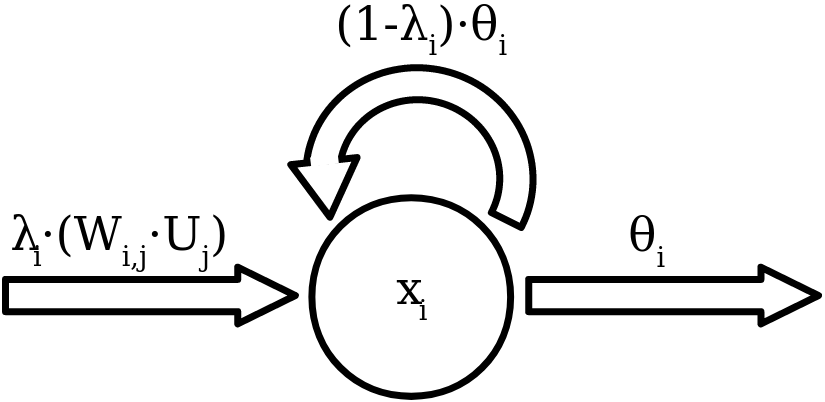
\includegraphics[width=.7\textwidth]{figures/leaky_integration.png}
%     \caption{Symbolic representation of a leaky integrating neuron.}
%     \label{fig:leaky_integration}
% \end{figure}

% This is an eps file, it is always sharp:\\
% Notice how the formatting option "[htbp]" allows for the figure to be moved around to page \pageref{fig:activation_function}. Hence, it is best to rather write: The eps file in figure \ref{fig:activation_function} always stays sharp.
% \begin{figure}[htbp]
%     \centering
%     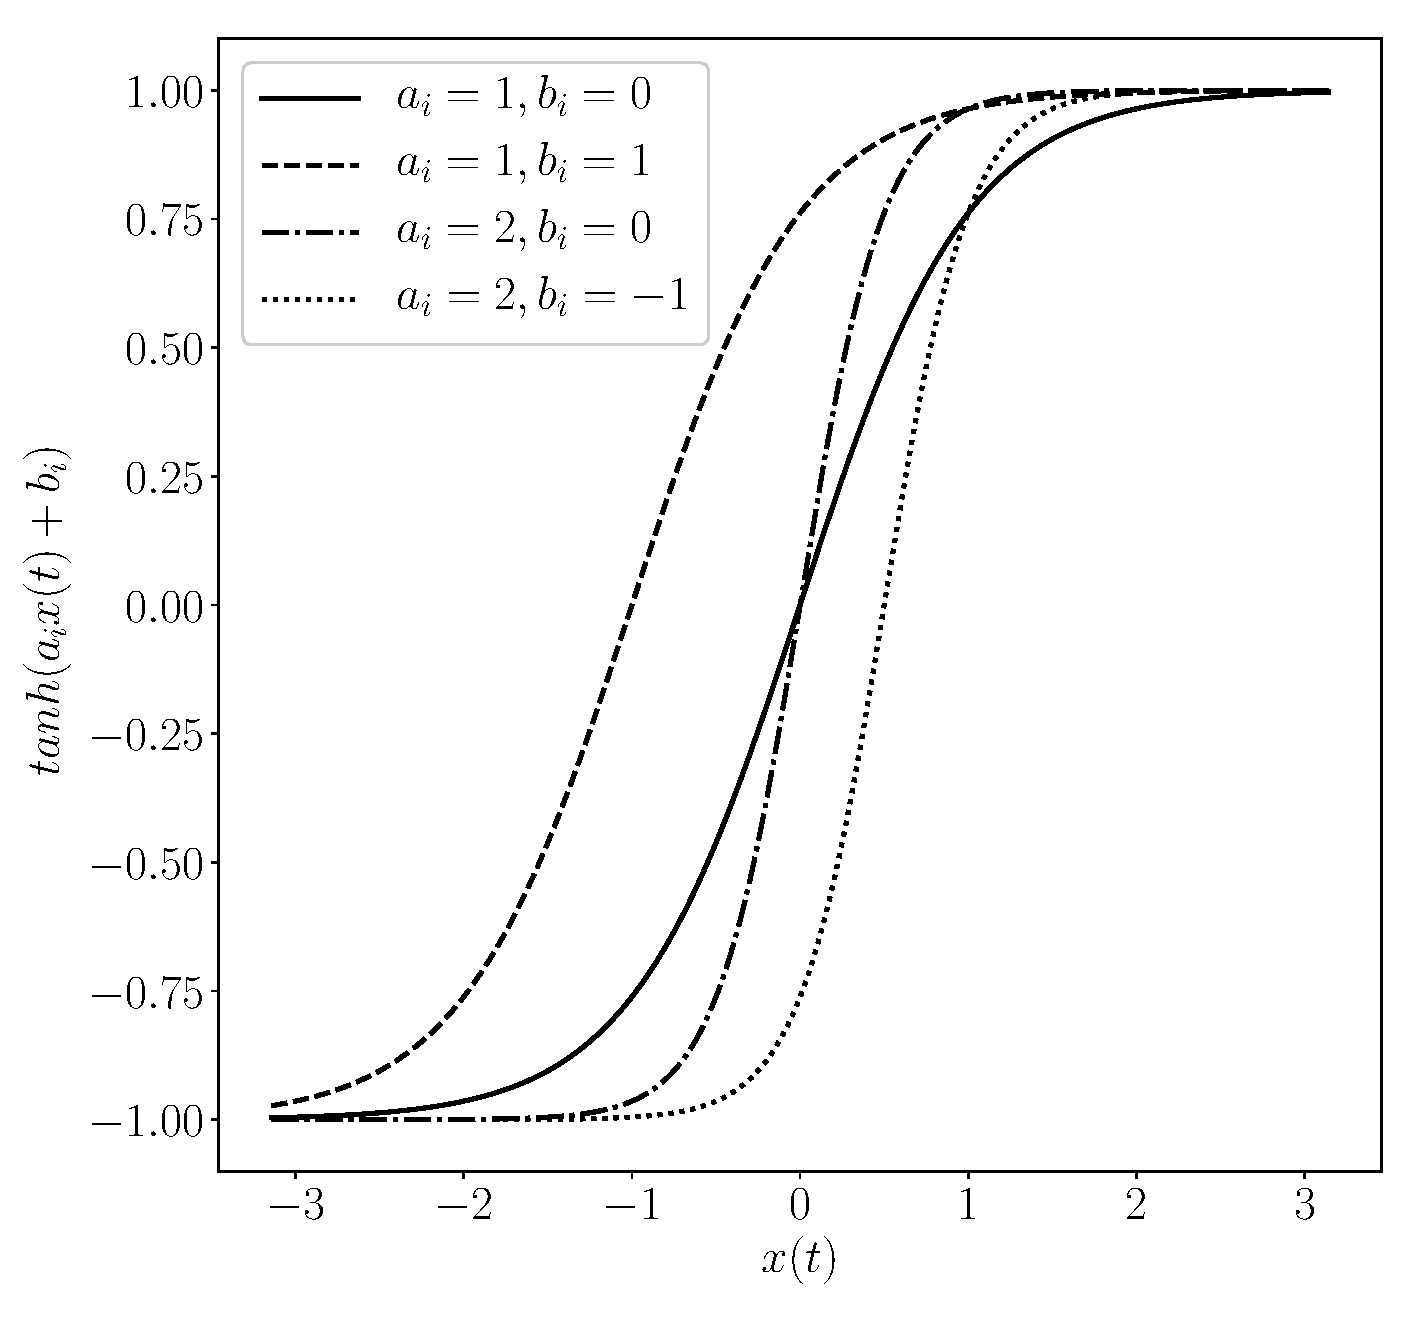
\includegraphics[width=.7\textwidth]{figures/activation_functions}
%     \caption{Shapes of a parametrized tanh activation function.}
%     \label{fig:activation_function}
% \end{figure}

% \subsection{Math example}
% The state update of the leaky integrating neuron in figure \ref{fig:leaky_integration} can be formulated as:
% \begin{align}
%     x_i(t+1) &= \lambda_i \cdot \left(W_{i,j} \cdot U_j(t)\right) + (1-\lambda_i) \cdot \theta_i(t)
%     \label{eq:leaky_integration}
% \end{align}

% \subsection{Code block example}
% From equation \ref{eq:leaky_integration} the neuron model is implemented using numpy \citep{harris:2020}:

% \lstinputlisting[label=py:leaky, language=Python, caption=Python implementation of a single leaky-integrating neuron.]{code/leaky.py}

% \subsection{Footnote example}
% The implementation is available on github\footnote{https://github.com/schniewmatz/recurrence}.
\newpage
\bibliography{bibliography}{}
\end{otherlanguage}
\end{document}
